\documentclass[11pt]{article}
\usepackage{fullpage}
\usepackage{enumitem}
\usepackage{pdfpages}
\usepackage{graphicx}
\usepackage{amsmath, amsthm}
\begin{document}
\author{Benjamin Sorenson} \title{Assignment 5}
\maketitle
\begin{enumerate}[label=\bfseries Question \arabic*:]
\item
  \begin{enumerate}
  \item
    \begin{align*}
      Action & (GoAndPick(x, y, o) \\
             & Precond: At(Robot, x) \land EmptyHand(Robot) \land At(o, y) \\
             & Effect: \lnot At(robot, x) \land At(Robot, y) \land \lnot EmptyHand(robot) \land \lnot At(o, y) \land Holding(Robot, o)) \\
    \end{align*}
  \item
    \begin{align*}
      Action & (PickAndGo(x, y, o) \\
             & Precond: At(Robot, x) \land EmptyHand(robot) \land At(o, x) \\ 
             & Effect: \lnot At(Robot, x) \land \lnot EmptyHand(Robot) \land \lnot At(o, x) \land Holding(Robot, o) \land At(Robot, y)) \\
    \end{align*}
  \item In general, action schemes can be combined by conjoining their
    preconditions and effects.  This can be useful useful when a
    conceptually single action may take several smaller actions to
    complete, but this may not be a good idea when the smaller
    component actions have more universal complexity. In this case, we
    may end up defining a lot of overly complex actions.
  \end{enumerate}
\item The action \(Go\)
  is unmodified, but \(Pick\)
  can be replaced with the following actions;
  \begin{align*}
    Action & (PickLeft(o, x)\\
           & Precond: EmptyLeftHand(Robot) \land At(Robot, x) \land At(o, x)\\
           & Effect: \lnot EmptyLeftHand(Robot) \land \lnot At(o, x) \land Holding(Robot, o)) \\
    \\
    Action & (PickRight(o, x)\\
           & Precond: EmptyRightHand(Robot) \land At(Robot, x) \land At(o, x)\\
           & Effect: \lnot EmptyRightHand(Robot) \land \lnot At(o, x) \land Holding(Robot, o)) \\
  \end{align*}
\item
  \begin{enumerate}
  \item
    \begin{align*}
      Action &(MoveTray(x, y) \\
             & Precond: At(Robot, x) \land At(Tray,y) \land EmptyHand(Robot) \\
             & Effect: \lnot At(Robot, x) \land \lnot At(Tray, x) \land At(Robot, y) \land At(Tray, x)) \\
      \\
      Action & (RemoveFromTray(o, x)\\ 
             & Precond: On(o, Tray) \land At(Tray, x) \land At(Robot, x) \land EmptyHand(Robot)\\
             & Effect: \lnot On(o, Tray))
    \end{align*}
  \item
    \begin{align*}
      Action & (RemoveGlassFromTray \\
             & Precond: GlassOnTray \land RobotInLivingRoom \land TrayInLivingRoom \land RobotHandEmpty \\
             & Effect: \lnot GlassOnTray)) \\
      \\ 
      Action & ( MoveTrayToKitchen\\
             & Precond: TrayInLivingRoom \land RobotInLivingRoom \land RobotHandEmpty\\
             & Effect: TrayInKitchen \land \lnot TrayInLivingRoom \land RobotInKitchen \land \lnot RobotInLivingRoom)
    \end{align*}
  \end{enumerate}
\item The predicate calculus allows variables, and proposition clculus
  does not.  In progpositional clculus we need a different fluent for
  each possible combination of variables which may become impractical
  as the number of variables becomes large.  While the predicate
  calculus allows variables, and thus has more expressive power than
  the propositional calculus, the propositional calculus is easier to
  analyze because each proposition is decidable.
\item
  \begin{enumerate}
  \item
    \begin{align*}
      Action & (CallElevatorFloor1\\
             & Precond: OnFloor1 \land AtElevatorFloor2\\
             & Effect: AtElevatorFloor1 \land \lnot AtElevatorFloor2)\\
      \\
      Action & (RideElevatorFLoor1\text{-}Floor2 \\
             & Precond: OnFloor1 \land AtElevatorFloor1\\
             & Effect: OnFloor2 \land \lnot OnFloor1 \land AtElevatorFloor2 \land \lnot AtElevatorFloor1)\\
    \end{align*}
  \item See last page ...
  \item The problem is solved at the second level.  The plan is
    \[CallElevatorFloor2 \rightarrow
    RideElevatorFloor2\text{-}Floor1\]
  \end{enumerate}
\item
  \begin{enumerate}
  \item If a literal does not appear in the final level of the
    planning graph it means that it is not a possible result of any
    action---if it were, it would persist to the final level.
  \item It is not necessary to add to the predecessor state the
    literals that are negative effects of the action because if the
    literal is a negative effect of the action, it could not have been
    negative in the predecessor state.
  \end{enumerate}
\end{enumerate}
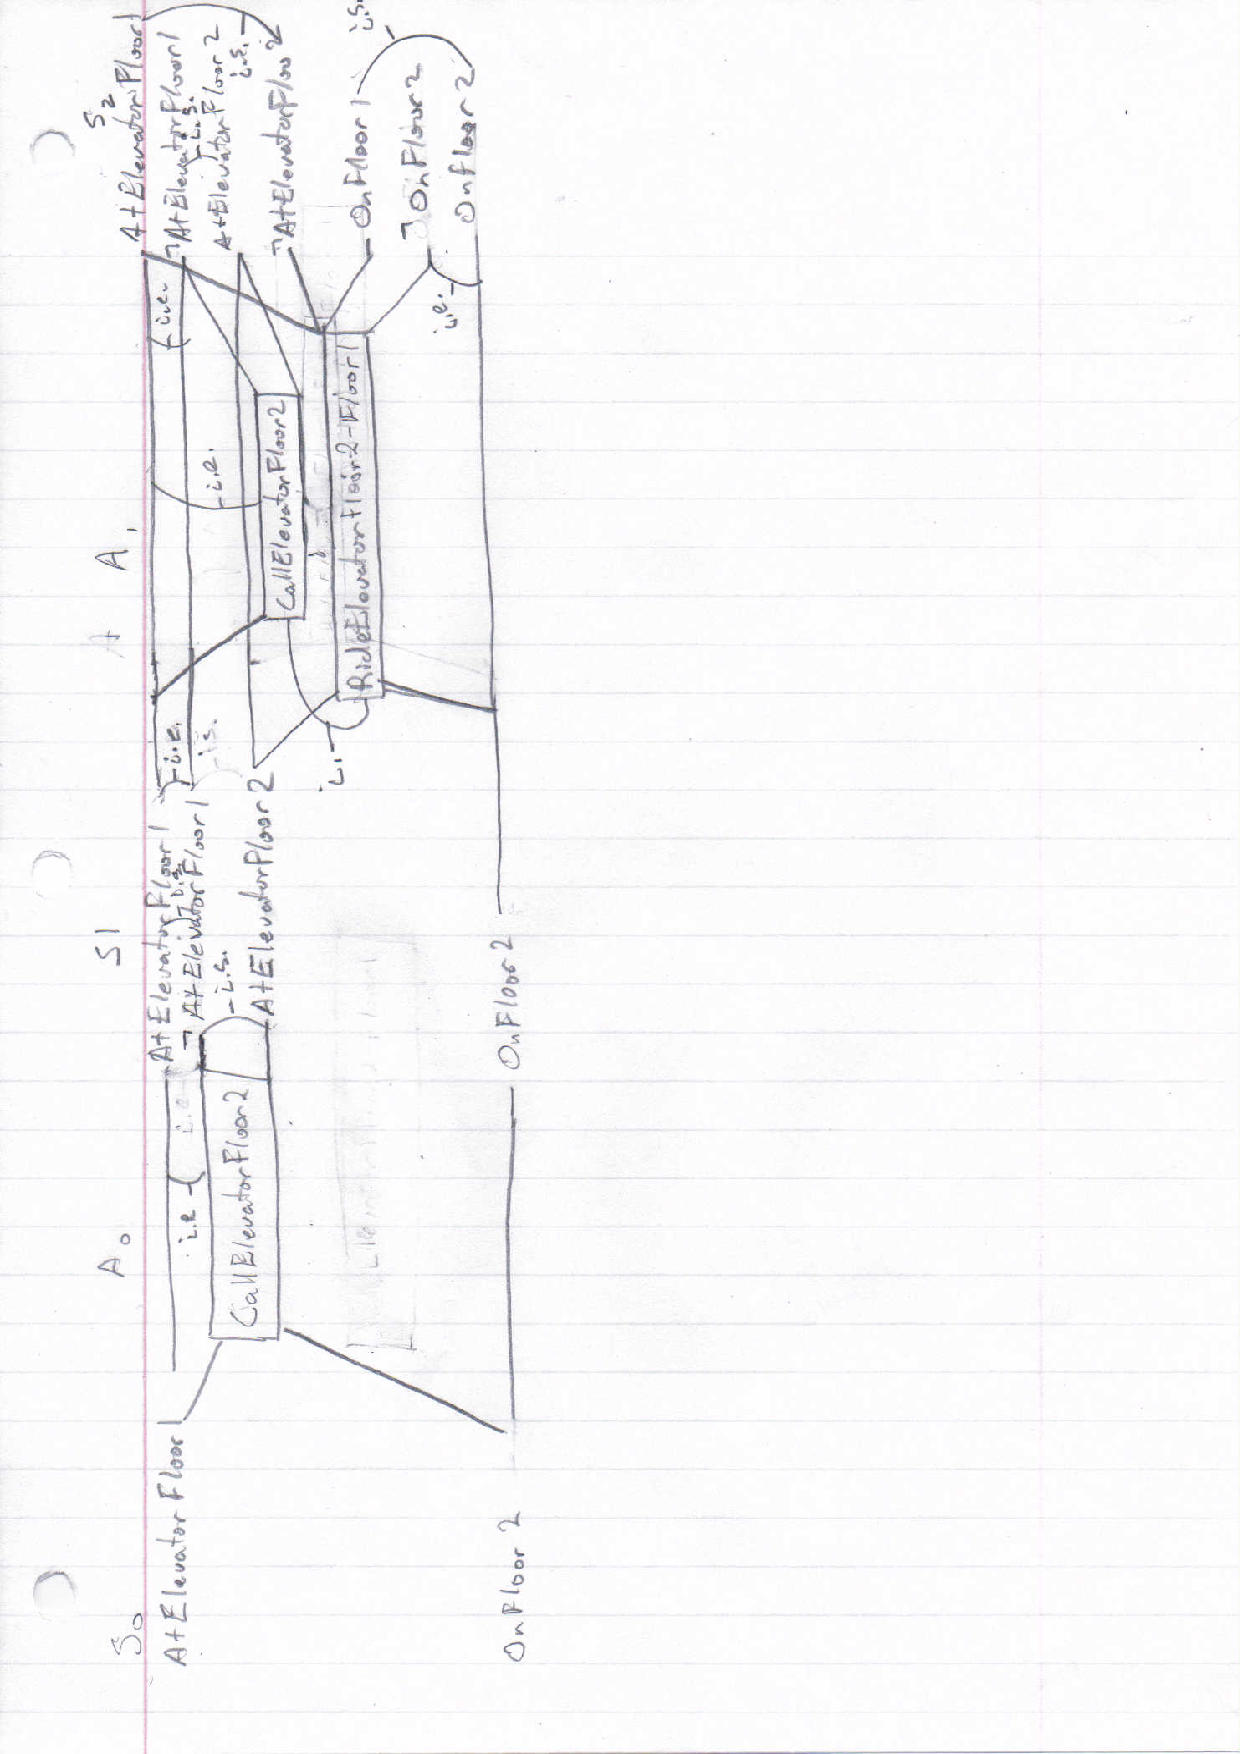
\includepdf{KSCN_10122015_3157.pdf}
\end{document}